% Created 2020-09-20 Sun 10:40
% Intended LaTeX compiler: xelatex
\documentclass[bigger,unknownkeysallowed,aspectratio=169,red,colorblocks]{beamer}
\usepackage{graphicx}
\usepackage{grffile}
\usepackage{minted}
\usepackage{longtable}
\usepackage{wrapfig}
\usepackage{rotating}
\usepackage[normalem]{ulem}
\usepackage{amsmath}
\usepackage{amssymb}
\usepackage{unicode-math}
\usepackage{mathtools}
\usepackage{textcomp}
\usepackage{capt-of}
\usepackage{hyperref}
\usepackage{minted}
\PassOptionsToPackage{unicode=true}{hyperref}
\PassOptionsToPackage{hyphens}{url}
\PassOptionsToPackage{dvipsnames,svgnames*,x11names*,table}{xcolor}
\usepackage{amssymb,amsmath}
\usepackage{mathtools}
\usepackage{physics}
\usepackage{hyperref}
\hypersetup{
pdftitle={Reproducible Scalable Workflows with Nix, Papermill and Renku},
pdfauthor={Rohit Goswami},
pdfborder={0 0 0},
breaklinks=true}
% Make use of float-package and set default placement for figures to H
\usepackage{float}
\floatplacement{figure}{H}
\usepackage{fontspec}
\setromanfont{EB Garamond}
\usefonttheme{serif}
\usepackage{xeCJK}
\usepackage[absolute,overlay]{textpos}
\newcommand*{\XOffsetFromBottomLeft}{32.5em}%
\newcommand*{\YOffsetFromBottomLeft}{2.7ex}%
\newcommand*{\BottomLeftText}[1]{%
\par%
\scriptsize\begin{textblock*}{17.0cm}(\dimexpr\textwidth-\XOffsetFromBottomLeft\relax,\dimexpr\textheight-\YOffsetFromBottomLeft\relax)
#1%
\end{textblock*}%
}%
\usepackage[doi=false,isbn=false,url=false,eprint=false]{biblatex}
\bibliography{IN2020.bib}
\setbeamertemplate{footnote}{%
\makebox[1em][l]{\insertfootnotemark}%
\begin{minipage}{\dimexpr\linewidth-1em}
\footnotesize\linespread{0.84}\selectfont\insertfootnotetext
\end{minipage}\vskip 0pt}%
\usetheme{Verona}
\author{Rohit Goswami,\textsc{\scriptsize\ MInstP AMIE AMIChemE}}
\date{October 3, 2020}
\title{Reproducible Scalable Workflows with Nix, Papermill and Renku}
\subtitle{PyCon India 2020}
\titlegraphic[height=1.5cm]{images/physUoI.png}{}
\mail{rog32@hi.is}
\hypersetup{
 pdfauthor={Rohit Goswami,\textsc{\scriptsize\ MInstP AMIE AMIChemE}},
 pdftitle={Reproducible Scalable Workflows with Nix, Papermill and Renku},
 pdfkeywords={},
 pdfsubject={},
 pdfcreator={Emacs 27.1 (Org mode 9.4)}, 
 pdflang={English}}
\begin{document}

\maketitle


\begin{frame}[label={sec:org464d316}]{Outline}
\begin{columns}
\begin{column}{0.5\columnwidth}
\tableofcontents
\end{column}
\begin{column}{0.5\columnwidth}
\begin{center}

\includegraphics[width=0.4\textwidth]{images/logos/pyConIN2020.png}
\end{center}
\end{column}
\end{columns}
\end{frame}
\begin{frame}[label={sec:org620b45b},standout]{Section I}
\section{Backstory}
\begin{center}
  \Huge Backstory
\end{center}
\end{frame}
\begin{frame}[label={sec:org3ff4a84}]{Standard Approach}
\begin{columns}
\begin{column}{0.5\columnwidth}
\begin{itemize}
\item Language Agnostic
\end{itemize}
\begin{block}{Workflow}
\begin{itemize}
\item Write functions/objects
\begin{itemize}
\item Refactor in modules
\end{itemize}
\item Test
\begin{itemize}
\item Unit
\item Integration
\end{itemize}
\item Documentation
\item Use after importing
\end{itemize}
\end{block}
\end{column}

\begin{column}{0.5\columnwidth}
\begin{center}

\includegraphics[width=0.8\textwidth]{images/Standard_Approach/2020-09-20_04-19-58_screenshot.png}
\end{center}
\end{column}
\end{columns}

\vspace{\fill}

\alert{Not interactive enough for data-files}
\end{frame}
\begin{frame}[label={sec:org407b254},fragile]{Modern Data Analysis}
 \begin{columns}
\begin{column}{0.5\columnwidth}
\begin{itemize}
\item Try before you buy
\item Doesn't play nice with tests
\end{itemize}
\begin{block}{Python Interactivity}
\begin{itemize}
\item IPython (\texttt{ipython})
\item Jupyter (Lab/Notebook)
\item Colab (Google)
\end{itemize}
\end{block}
\end{column}
\begin{column}{0.5\columnwidth}
\begin{center}
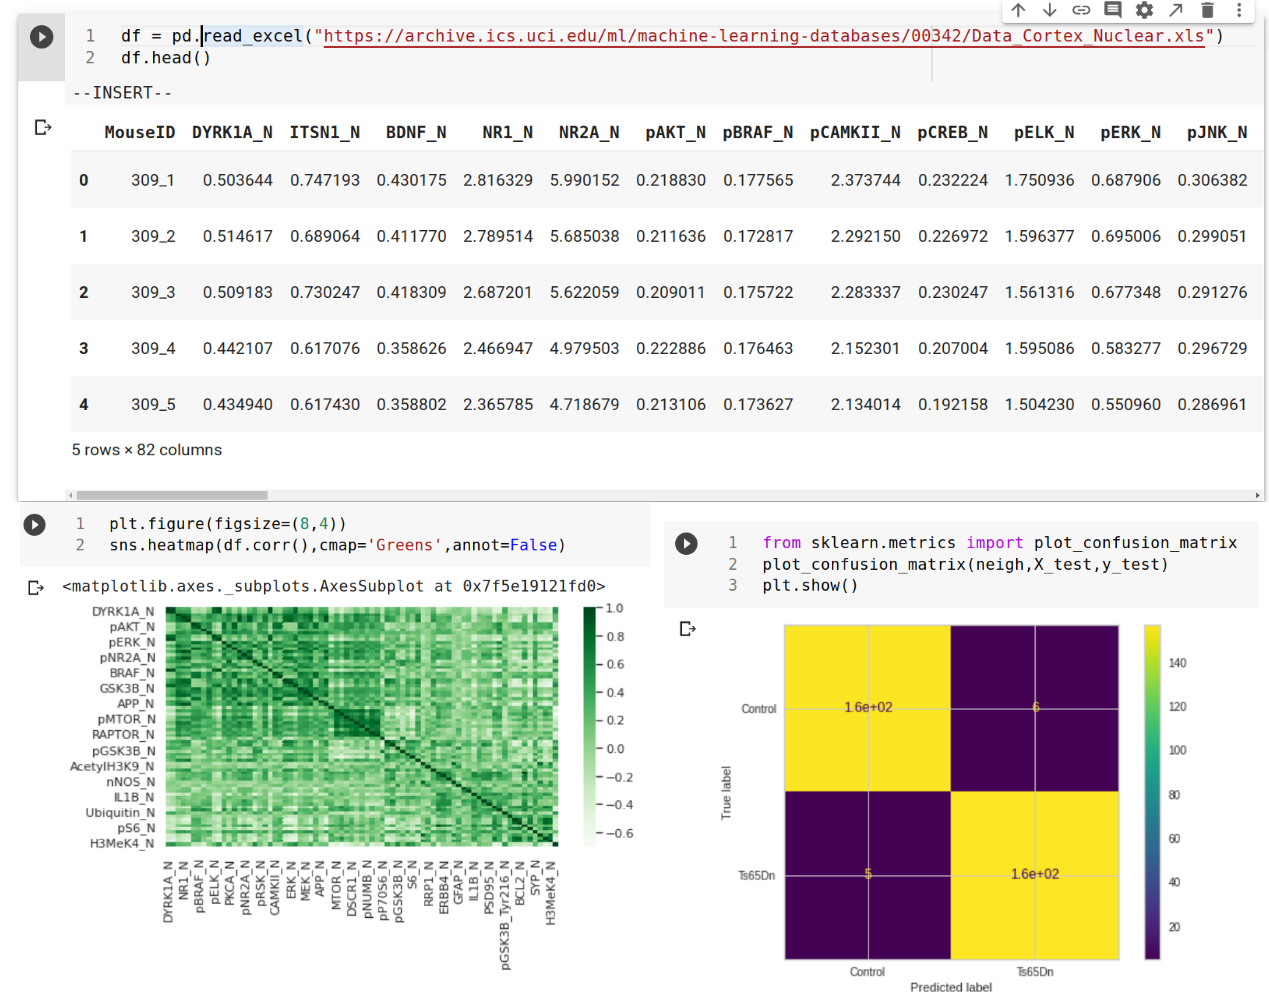
\includegraphics[width=.9\linewidth]{images/Modern_Data_Analysis/2020-09-20_04-32-08_screenshot.png}
\end{center}
\end{column}
\end{columns}
\end{frame}

\begin{frame}[label={sec:org194be2e}]{Jupyter}
\begin{columns}
\begin{column}{0.4\columnwidth}
\fullcite{communityTuringWayHandbook2019}

\begin{center}

\includegraphics[width=.9\linewidth]{images/A_block/2020-09-20_04-38-32_screenshot.png}
\end{center}
\end{column}

\begin{column}{0.6\columnwidth}
\begin{center}
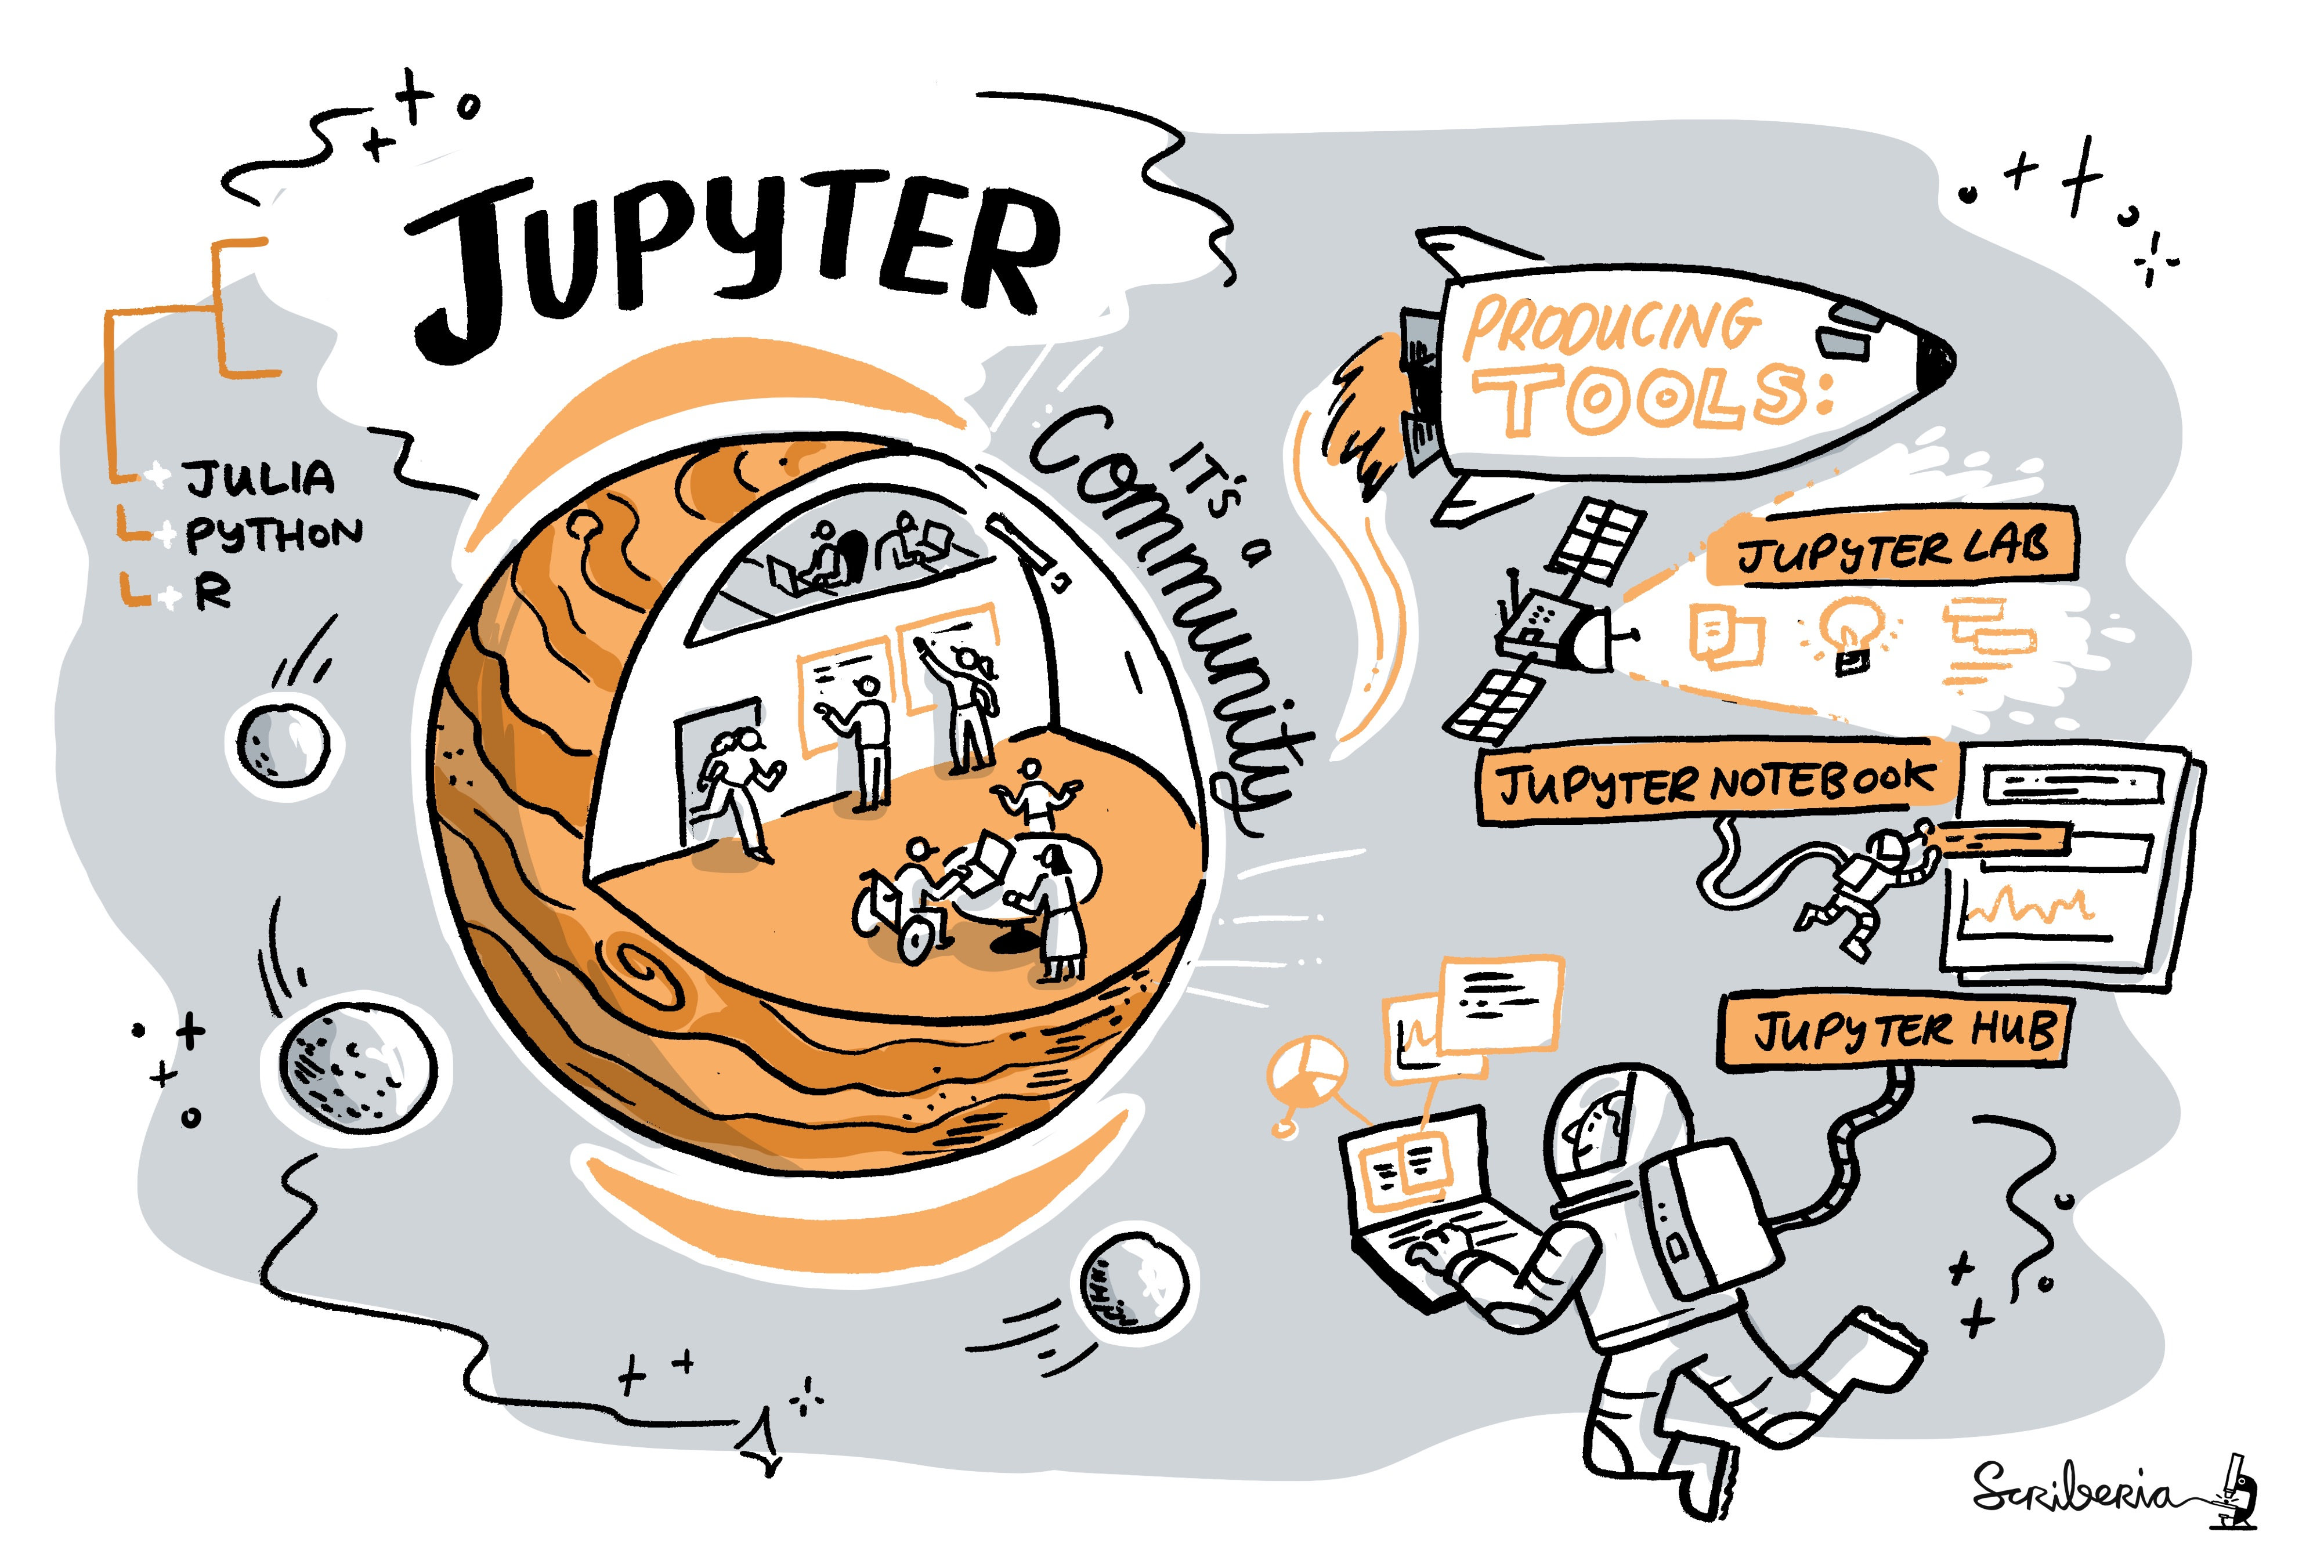
\includegraphics[width=.9\linewidth]{images/turingWay/Jupyter.jpg}
\end{center}
\end{column}
\end{columns}
\end{frame}
\begin{frame}[label={sec:org58a9aef},fragile]{Jupyter Notebooks}
 \begin{columns}
\begin{column}{0.5\columnwidth}
\begin{itemize}
\item \texttt{ipynb} files can be exported independently
\begin{itemize}
\item Or via server extensions
\end{itemize}
\end{itemize}
\begin{center}
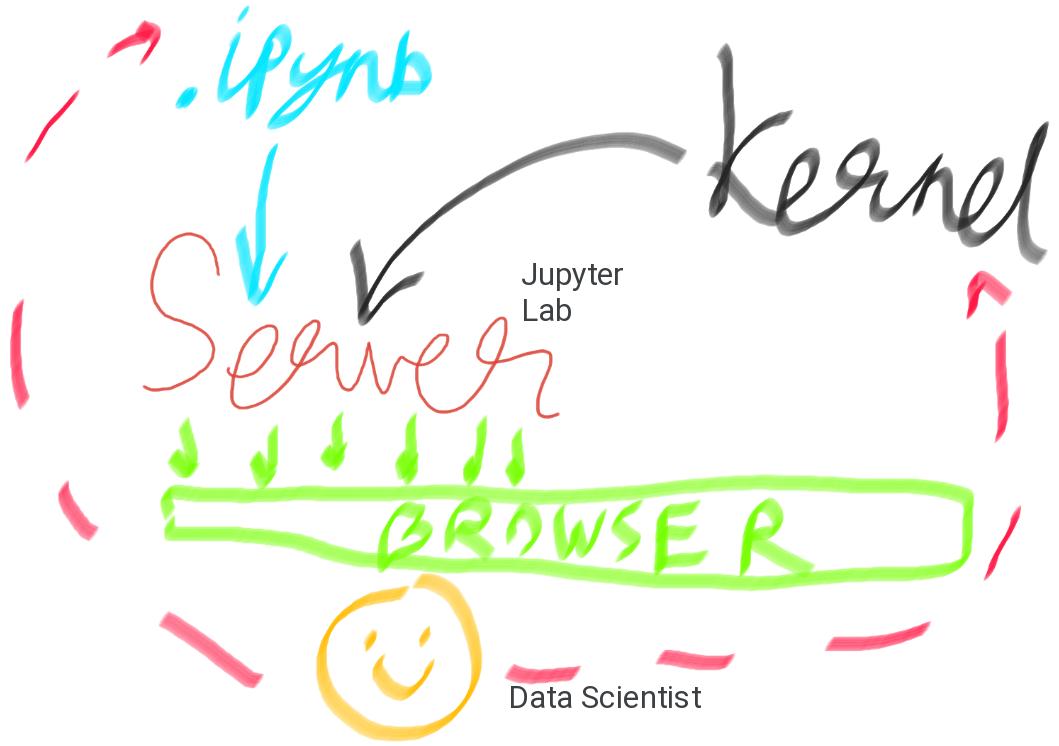
\includegraphics[width=.9\linewidth]{images/A_block/2020-09-20_10-34-58_screenshot.png}
\end{center}
\end{column}

\begin{column}{0.5\columnwidth}
\begin{center}
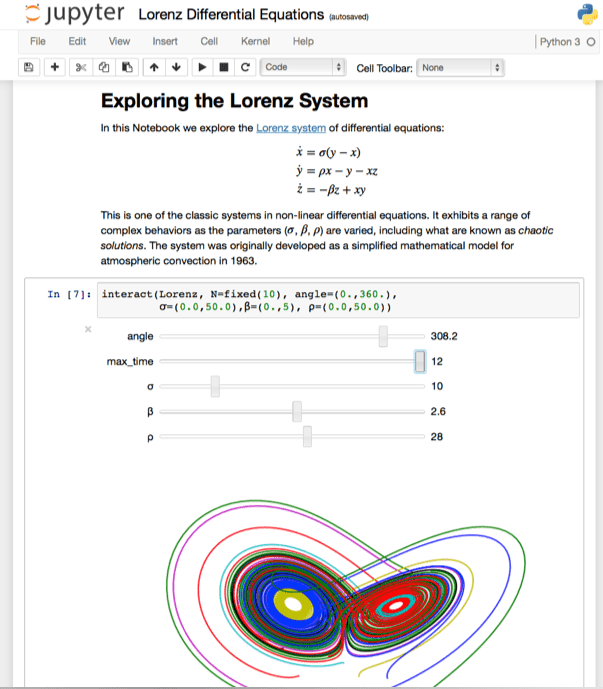
\includegraphics[width=0.7\textwidth]{images/A_screenshot/2020-09-20_09-14-03_screenshot.png}
\end{center}
\end{column}
\end{columns}

From \href{https://jupyter.readthedocs.io/en/latest/projects/architecture/content-architecture.html}{the Jupyter documentation}
\end{frame}
\begin{frame}[label={sec:org03b941f}]{Reconciliation}
\begin{columns}
\begin{column}{0.3\columnwidth}
\begin{itemize}
\item A crisis of \alert{faith}
\item Made worse by Colab
\end{itemize}
\end{column}

\begin{column}{0.7\columnwidth}
\begin{center}
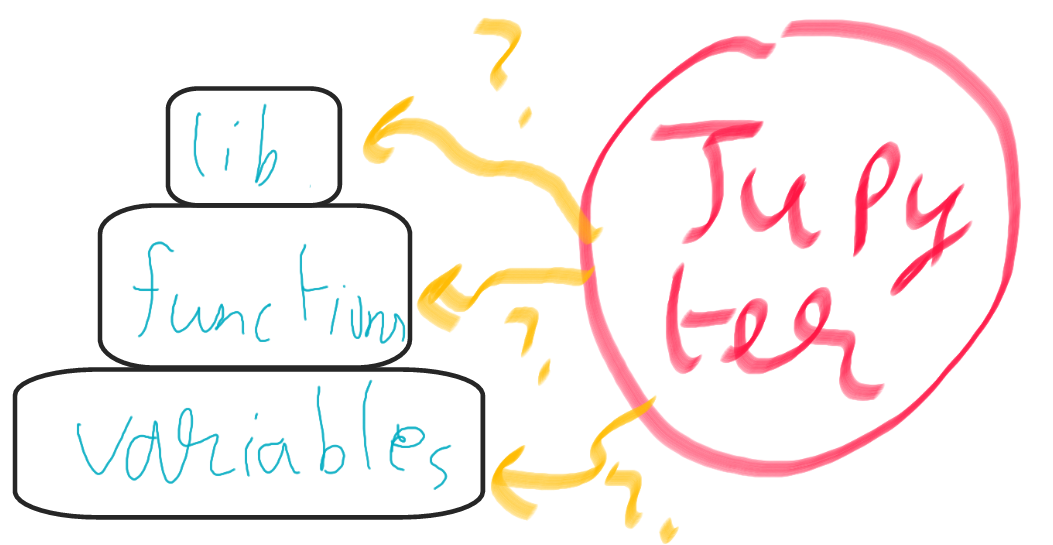
\includegraphics[width=.9\linewidth]{images/Reconciliation/2020-09-20_06-18-07_screenshot.png}
\end{center}
\end{column}
\end{columns}
\end{frame}

\begin{frame}[label={sec:orgdca0415},standout]{Section II}
\section{Packaging}
\begin{center}
  \Huge Packaging
\end{center}
\end{frame}
\begin{frame}[label={sec:org6bf903a},fragile]{Python Modules}
 \begin{itemize}
\item A \texttt{.py} file is a \alert{module}
\item It is \alert{standalone} if it only imports from the standard library
\end{itemize}
\end{frame}
\begin{frame}[label={sec:org56253ba},fragile]{Pure Python Packages}
 \begin{itemize}
\item A directory with \texttt{\_\_init\_\_.py} in it is a \alert{package}
\item Use \texttt{pip}
\end{itemize}
\end{frame}
\begin{frame}[label={sec:orgde819f4},fragile]{Distributions}
 \begin{columns}
\begin{column}{0.45\columnwidth}
\begin{block}{Standard}
\begin{itemize}
\item Built by \texttt{setuptools} with \texttt{setup.py}
\item Simple source only \texttt{.tar.gz}
\end{itemize}
\end{block}
\end{column}
\begin{column}{0.45\columnwidth}
\begin{block}{Binary}
\begin{itemize}
\item \texttt{wheel}
\begin{itemize}
\item For all your interoperable needs
\item Includes static libraries
\end{itemize}
\end{itemize}
\end{block}
\end{column}
\end{columns}
\begin{itemize}
\item Distributions have zero or more packages
\end{itemize}
\end{frame}
\begin{frame}[label={sec:orgf12e1dc}]{The Python Gradient}
Consider the packaging gradient\footnotemark
\begin{center}
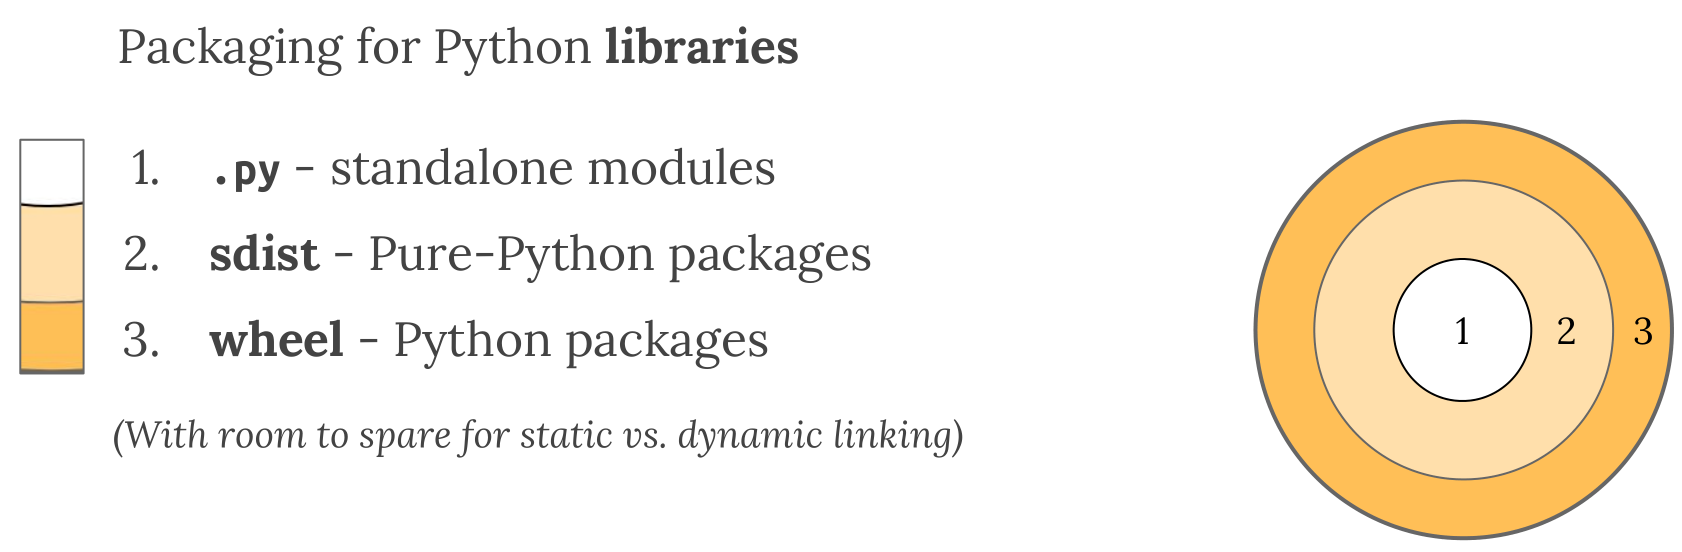
\includegraphics[width=.9\linewidth]{images/The_Python_Gradient/2020-05-22_23-00-30_screenshot.png}
\end{center}
\begin{itemize}
\item Libraries and Dev tools are all we get (from PyPI)
\end{itemize}

\footnotetext{by Mahmoud Hashemi (PyBay'17): \url{https://www.youtube.com/watch?v=iLVNWfPWAC8}}
\end{frame}
\begin{frame}[label={sec:org441c074}]{Pip Requirements}
\begin{itemize}
\item Python
\item System libraries
\item Build tools
\begin{itemize}
\item Wheels don't work for arbitrary distributions
\end{itemize}
\end{itemize}
\end{frame}
\begin{frame}[label={sec:org9332c10},fragile]{Dependency Resolution}
 \begin{columns}
\begin{column}{0.5\columnwidth}
\begin{itemize}
\item \texttt{requirements.txt} (pip)
\item Poetry (pretty)
\begin{itemize}
\item \texttt{pyproject.toml}
\item \texttt{poetry.lock}
\end{itemize}
\item Pipenv (older)
\begin{itemize}
\item \texttt{Pipfile} + lockfile
\end{itemize}
\item Pipx (\texttt{pip} but for applications)
\item Pyenv and friends
\end{itemize}
\end{column}
\begin{column}{0.5\columnwidth}
\begin{center}

\includegraphics[width=0.6\textwidth]{images/Dependency_Resolution/2020-09-20_05-09-56_screenshot.png}
\end{center}
\end{column}
\end{columns}
\end{frame}
\begin{frame}[label={sec:org67540f1},fragile]{System Dependencies}
 \begin{columns}
\begin{column}{0.5\columnwidth}
\begin{itemize}
\item Appimages
\item Containers
\begin{itemize}
\item \texttt{docker}, \texttt{flatpak}, \texttt{snapcraft}
\end{itemize}
\item Impure filesystems
\begin{itemize}
\item Anaconda
\end{itemize}
\end{itemize}
\end{column}
\begin{column}{0.5\columnwidth}
\begin{center}

\includegraphics[width=0.6\textwidth]{images/System_Dependencies/2020-09-20_05-23-11_screenshot.png}
\end{center}
\end{column}
\end{columns}
\end{frame}

\begin{frame}[label={sec:org9c20a44},standout]{Section III}
\section{Nix}
\begin{center}
  \Huge Nix
\end{center}
\end{frame}
\begin{frame}[label={sec:org5ca6ba0}]{What?}
\begin{center}
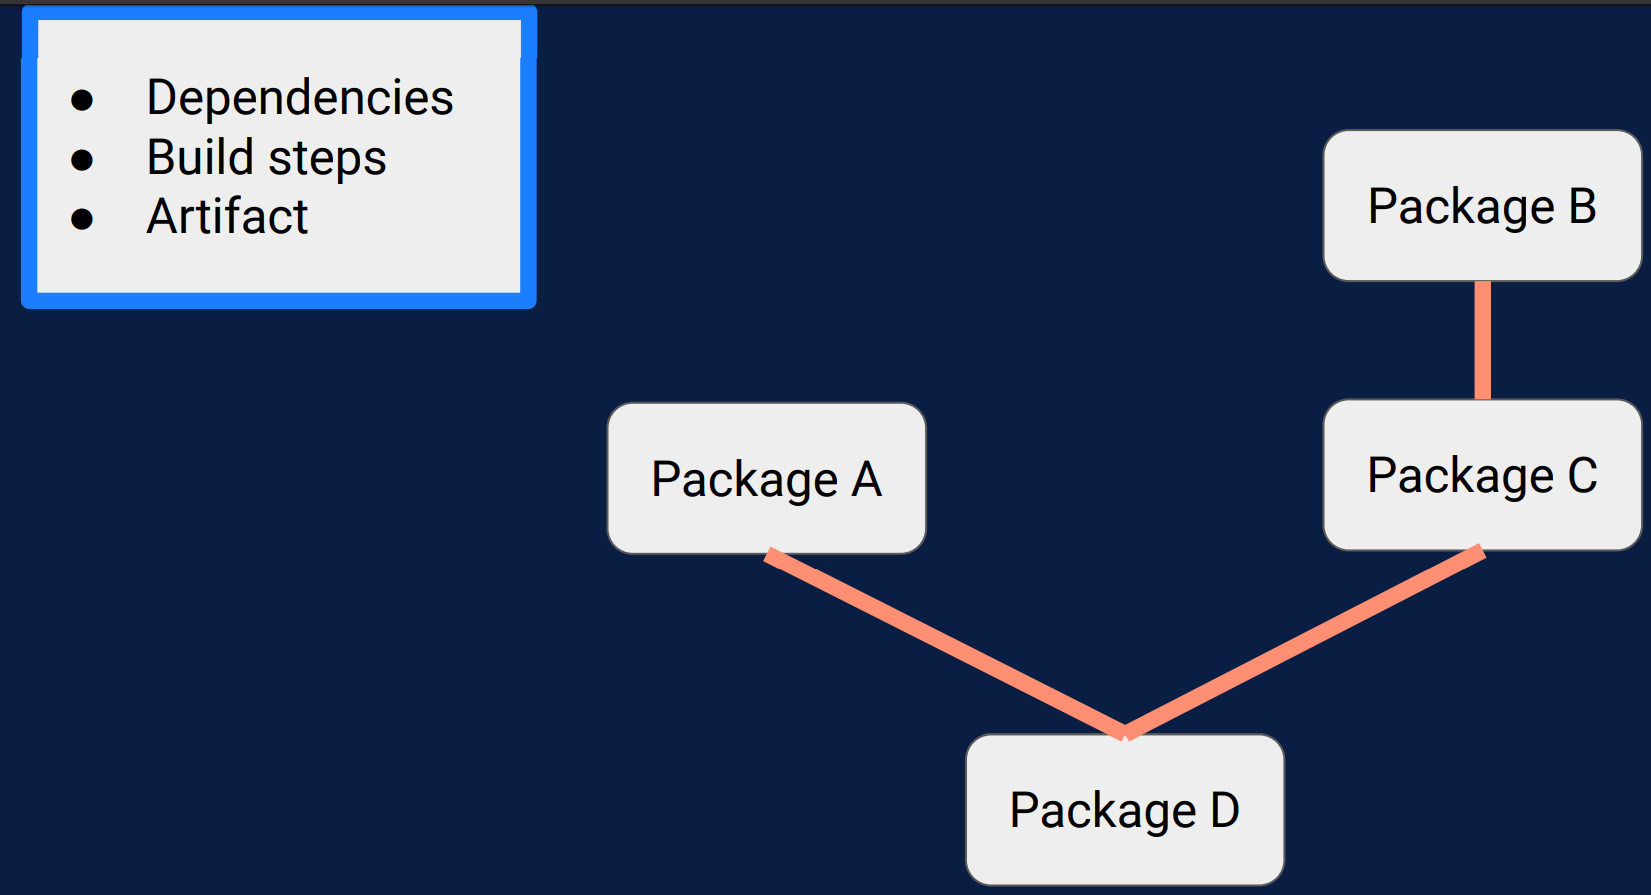
\includegraphics[width=0.5\linewidth]{images/What?/2020-05-22_23-04-53_screenshot.png}
\end{center}
\begin{itemize}
\item \tiny from \url{https://brianmckenna.org/files/presentations/rootconf19-nix.pdf}
\end{itemize}
\end{frame}
\begin{frame}[label={sec:org080a46e}]{Nix}
\begin{columns}
\begin{column}{0.4\columnwidth}
\fullcite{dolstraNixSafePolicyFree2004,dolstraNixOSPurelyFunctional2010}
\end{column}

\begin{column}{0.6\columnwidth}
\begin{center}
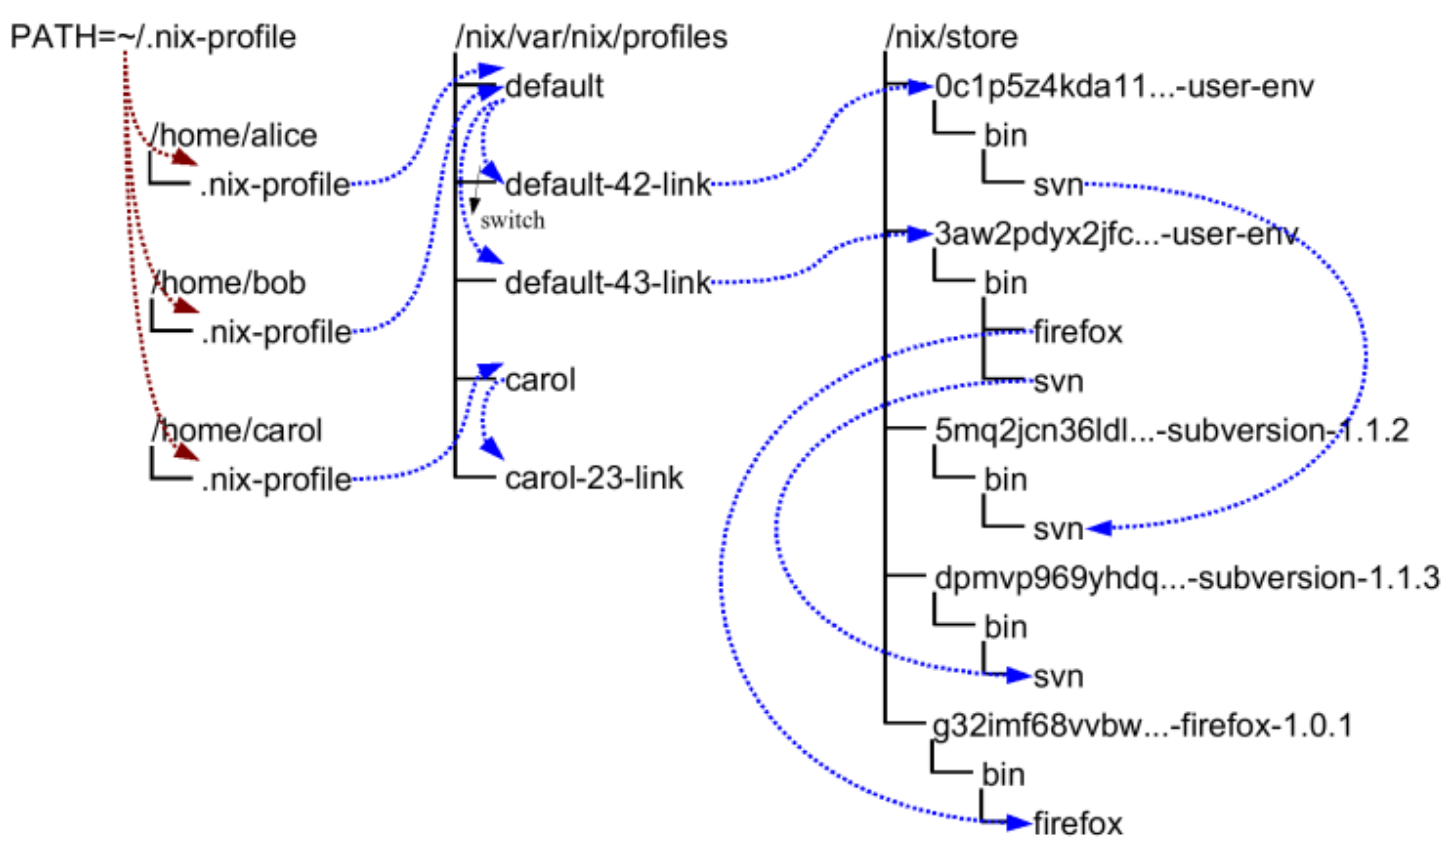
\includegraphics[width=.9\linewidth]{images/A_screenshot/2020-05-22_23-15-22_screenshot.png}
\end{center}
\end{column}
\end{columns}
\end{frame}
\begin{frame}[label={sec:org3aee92a}]{Why?}
\begin{columns}
\begin{column}{0.4\columnwidth}
\begin{quote}
Protects against self harm
\end{quote}
\begin{quote}
Exposes things taken for granted
\end{quote}
\begin{quote}
Enforces consistency
\end{quote}
\end{column}
\begin{column}{0.6\columnwidth}
\begin{description}
\item[{Reliable}] Purely functional, no broken dependencies
\item[{Reproducible}] Each package is in isolation
\item[{How?}] store + hash + name + version
\end{description}
\end{column}
\end{columns}
\end{frame}
\begin{frame}[label={sec:orge4c4ebc},fragile]{Installation (Multi-User)}
 \begin{minted}[bgcolor=white,breaklines=true,linenos=true,style=tango]{bash}
sh <(curl https://nixos.org/nix/install) --daemon
\end{minted}

\begin{itemize}
\item Needs \texttt{sudo} but should not be run as root
\item Will make build users with IDs between 30001 and 30032 along with a group ID 30000
\end{itemize}
\end{frame}
\begin{frame}[label={sec:orgff2b6fc},fragile]{Nix Python - Trial I}
 \begin{minted}[bgcolor=white,breaklines=true,linenos=true,style=tango]{bash}
nix-shell -p 'python38.withPackages(ps: with ps; [ numpy toolz ])'
\end{minted}

\begin{itemize}
\item Check which \texttt{python} is loaded
\item Check which modules are present
\end{itemize}
\end{frame}
\begin{frame}[label={sec:org2dd43b0},fragile]{Nix with Scripts}
 \begin{minted}[bgcolor=white,breaklines=true,linenos=true,style=tango]{bash}
#! /usr/bin/env nix-shell
#! nix-shell -i python3 -p "python3.withPackages(ps: [ps.numpy])"

import numpy

print(numpy.__version__)
\end{minted}
\end{frame}
\begin{frame}[label={sec:org7f75524},fragile]{An Aside into Purity}
 \begin{columns}
\begin{column}{0.4\columnwidth}
\begin{minted}[bgcolor=white,breaklines=true,linenos=true,style=tango]{bash}
nix-shell --pure --run 'bash'
\end{minted}
\begin{itemize}
\item Why?
\item What do we solve with this?
\end{itemize}
\end{column}

\begin{column}{0.6\columnwidth}
\begin{figure}[htbp]
\centering
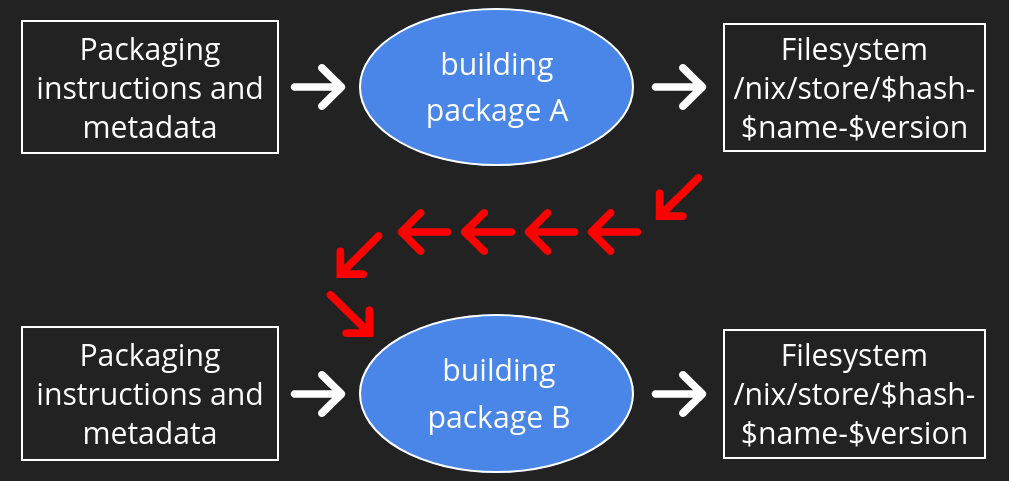
\includegraphics[width=.9\linewidth]{images/A_screenshot/2020-05-22_23-57-17_screenshot.png}
\caption{Stateless builds from \url{https://slides.com/garbas/mozilla-all-hands-london-2016\#/7/0/3}}
\end{figure}
\end{column}
\end{columns}
\end{frame}

\begin{frame}[label={sec:orgabdb45b},fragile]{Shell in a File}
 \begin{columns}
\begin{column}{0.6\columnwidth}
\begin{minted}[bgcolor=white,breaklines=true,linenos=true,style=tango]{nix}
with import <nixpkgs> {};

let
  pythonEnv = python35.withPackages (ps: [
    ps.numpy
    ps.toolz
  ]);
in mkShell {
  buildInputs = [
    pythonEnv
    which
  ];}
\end{minted}
\end{column}
\begin{column}{0.4\columnwidth}
\begin{itemize}
\item What \alert{tools} are we adding?
\item What \alert{environment} are we using?
\end{itemize}
\end{column}
\end{columns}
\end{frame}
\begin{frame}[label={sec:orgf23eadc},fragile]{Nix Python Expressions I}
 \begin{columns}
\begin{column}{0.6\columnwidth}
\begin{minted}[bgcolor=white,breaklines=true,linenos=true,style=tango]{nix}
f90wrap = self.buildPythonPackage rec {
  pname = "f90wrap";
  version = "0.2.3";
  src = pkgs.fetchFromGitHub {
    owner = "jameskermode";
    repo = "f90wrap";
    rev = "master";
    sha256 = "0d06nal4xzg8vv6sjdbmg2n88a8h8df5ajam72445mhzk08yin23";
  };
  buildInputs = with pkgs; [ gfortran stdenv ];
\end{minted}
\end{column}

\begin{column}{0.4\columnwidth}
\begin{itemize}
\item The self portion is from overriding the python environment
\item We will dispense with this later
\end{itemize}
\end{column}
\end{columns}
\end{frame}
\begin{frame}[label={sec:org2f4df6e},fragile]{Nix Python Expressions II}
 \begin{columns}
\begin{column}{0.6\columnwidth}
\begin{minted}[bgcolor=white,breaklines=true,linenos=true,style=tango]{nix}
  propagatedBuildInputs = with self; [
    setuptools
    setuptools-git
    wheel
    numpy
  ];
  preConfigure = ''
    export F90=${pkgs.gfortran}/bin/gfortran
  '';
  doCheck = false;
  doIstallCheck = false;
};
\end{minted}
\end{column}
\begin{column}{0.4\columnwidth}
\begin{itemize}
\item More details here: \url{https://rgoswami.me/posts/ccon-tut-nix/}
\item Note that the \texttt{propagatedBuildInputs} are for the python packages
\end{itemize}
\end{column}
\end{columns}
\end{frame}
\begin{frame}[label={sec:org5c692ad},fragile]{Friendly Nix}
 \begin{columns}
\begin{column}{0.4\columnwidth}
\begin{minted}[bgcolor=white,breaklines=true,linenos=true,style=tango]{bash}
nix-env -i nox
nox niv
\end{minted}
\end{column}
\begin{column}{0.6\columnwidth}
\begin{description}
\item[{Niv}] For pinning packages
\item[{Nox}] Interactive package management
\item[{\href{https://github.com/target/lorri/}{Lorri}}] For automatically reloading environments
\item[{Mach-Nix}] For working with Python
\item[{Nix-Prefetch-Url}] For obtaining SHA hashes
\end{description}
\end{column}
\end{columns}
\end{frame}
\begin{frame}[label={sec:orgb4c1138},standout]{Section IV}
\section{Setup}
\begin{center}
  \Huge Setup
\end{center}
\end{frame}
\begin{frame}[label={sec:orgc03a098},fragile]{Replacing Conda I}
 \begin{columns}
\begin{column}{0.6\columnwidth}
\begin{minted}[bgcolor=white,breaklines=true,linenos=true,style=tango]{nix}
let
  sources = import ./prjSource/nix/sources.nix;
  pkgs = import sources.nixpkgs { };
  mach-nix = import (builtins.fetchGit {
    url = "https://github.com/DavHau/mach-nix/";
    ref = "2.2.2";
  });
\end{minted}
\end{column}

\begin{column}{0.4\columnwidth}
\begin{itemize}
\item Note our definition of \texttt{mach-nix}
\item Best practices involve \texttt{niv} pinned sources
\end{itemize}
\end{column}
\end{columns}
\end{frame}
\begin{frame}[label={sec:org8ad2749},fragile]{Replacing Conda II}
 \begin{columns}
\begin{column}{0.6\columnwidth}
\begin{minted}[bgcolor=white,breaklines=true,linenos=true,style=tango]{nix}
  customPython = mach-nix.mkPython {
    requirements = builtins.readFile ./requirements.txt;
    providers = {
      _default = "nixpkgs,wheel,sdist";
      pytest = "nixpkgs";
    };
    pkgs = pkgs;
  };
in pkgs.mkShell { buildInputs = with pkgs; [ customPython ]; }
\end{minted}
\end{column}
\begin{column}{0.4\columnwidth}
\begin{itemize}
\item More details here: \url{https://rgoswami.me/posts/mach-nix-niv-python/}
\end{itemize}
\end{column}
\end{columns}
\end{frame}
\begin{frame}[label={sec:org0cf1eec},fragile]{Replacing Conda III}
 \begin{columns}
\begin{column}{0.6\columnwidth}
\begin{minted}[bgcolor=white,breaklines=true,linenos=true,style=tango]{nix}
    overrides_pre = [
      (pythonSelf: pythonSuper: {
        pytest = pythonSuper.pytest.overrideAttrs (oldAttrs: {
          doCheck = false;
        });
        f90wrap = pythonSelf.buildPythonPackage rec {...};
      })
    ];
\end{minted}
\end{column}
\begin{column}{0.4\columnwidth}
\begin{itemize}
\item An important aspect of \texttt{mkPython}
\item More details here: \url{https://rgoswami.me/posts/mach-nix-niv-python/}
\end{itemize}
\end{column}
\end{columns}
\end{frame}
\begin{frame}[label={sec:org49b51d2}]{More Nix}
\begin{columns}
\begin{column}{0.6\columnwidth}
\begin{itemize}
\item Try \href{https://nixos.org/nixos/nix-pills/why-you-should-give-it-a-try.html}{Nix Pills}
\item Roll your own environment
\item Make a docker image
\item Try a more \href{https://github.com/d-SEAMS/seams-core/blob/691da72262db40625774a2aed05d23c17a211360/nix/pkgs/sharkML/sharkML.nix}{complex system} (\href{https://dseams.info}{d-SEAMS} \cite{goswamiDSEAMSDeferredStructural2020})
\end{itemize}
\end{column}
\begin{column}{0.4\columnwidth}
\begin{center}
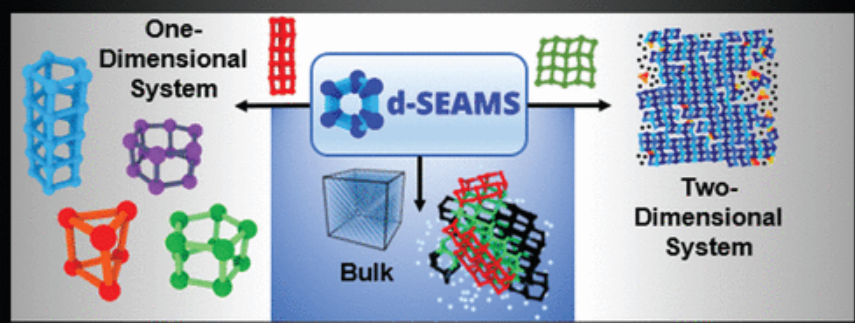
\includegraphics[width=.9\linewidth]{images/A_screenshot/2020-05-22_23-54-29_screenshot.png}
\end{center}
\end{column}
\end{columns}
\end{frame}

\begin{frame}[label={sec:orgb514a7e},standout]{Section V}
\section{Reproducibility}
\begin{center}
  \Huge Reproducibility
\end{center}
\end{frame}
\begin{frame}[label={sec:org91b8ea8}]{What Reproducibility?}
\begin{columns}
\begin{column}{0.4\columnwidth}
\fullcite{communityTuringWayHandbook2019}

\begin{center}

\includegraphics[width=0.4\textwidth]{images/turingWay/LogoDetailWithText.jpg}
\end{center}
\end{column}

\begin{column}{0.6\columnwidth}
\begin{center}
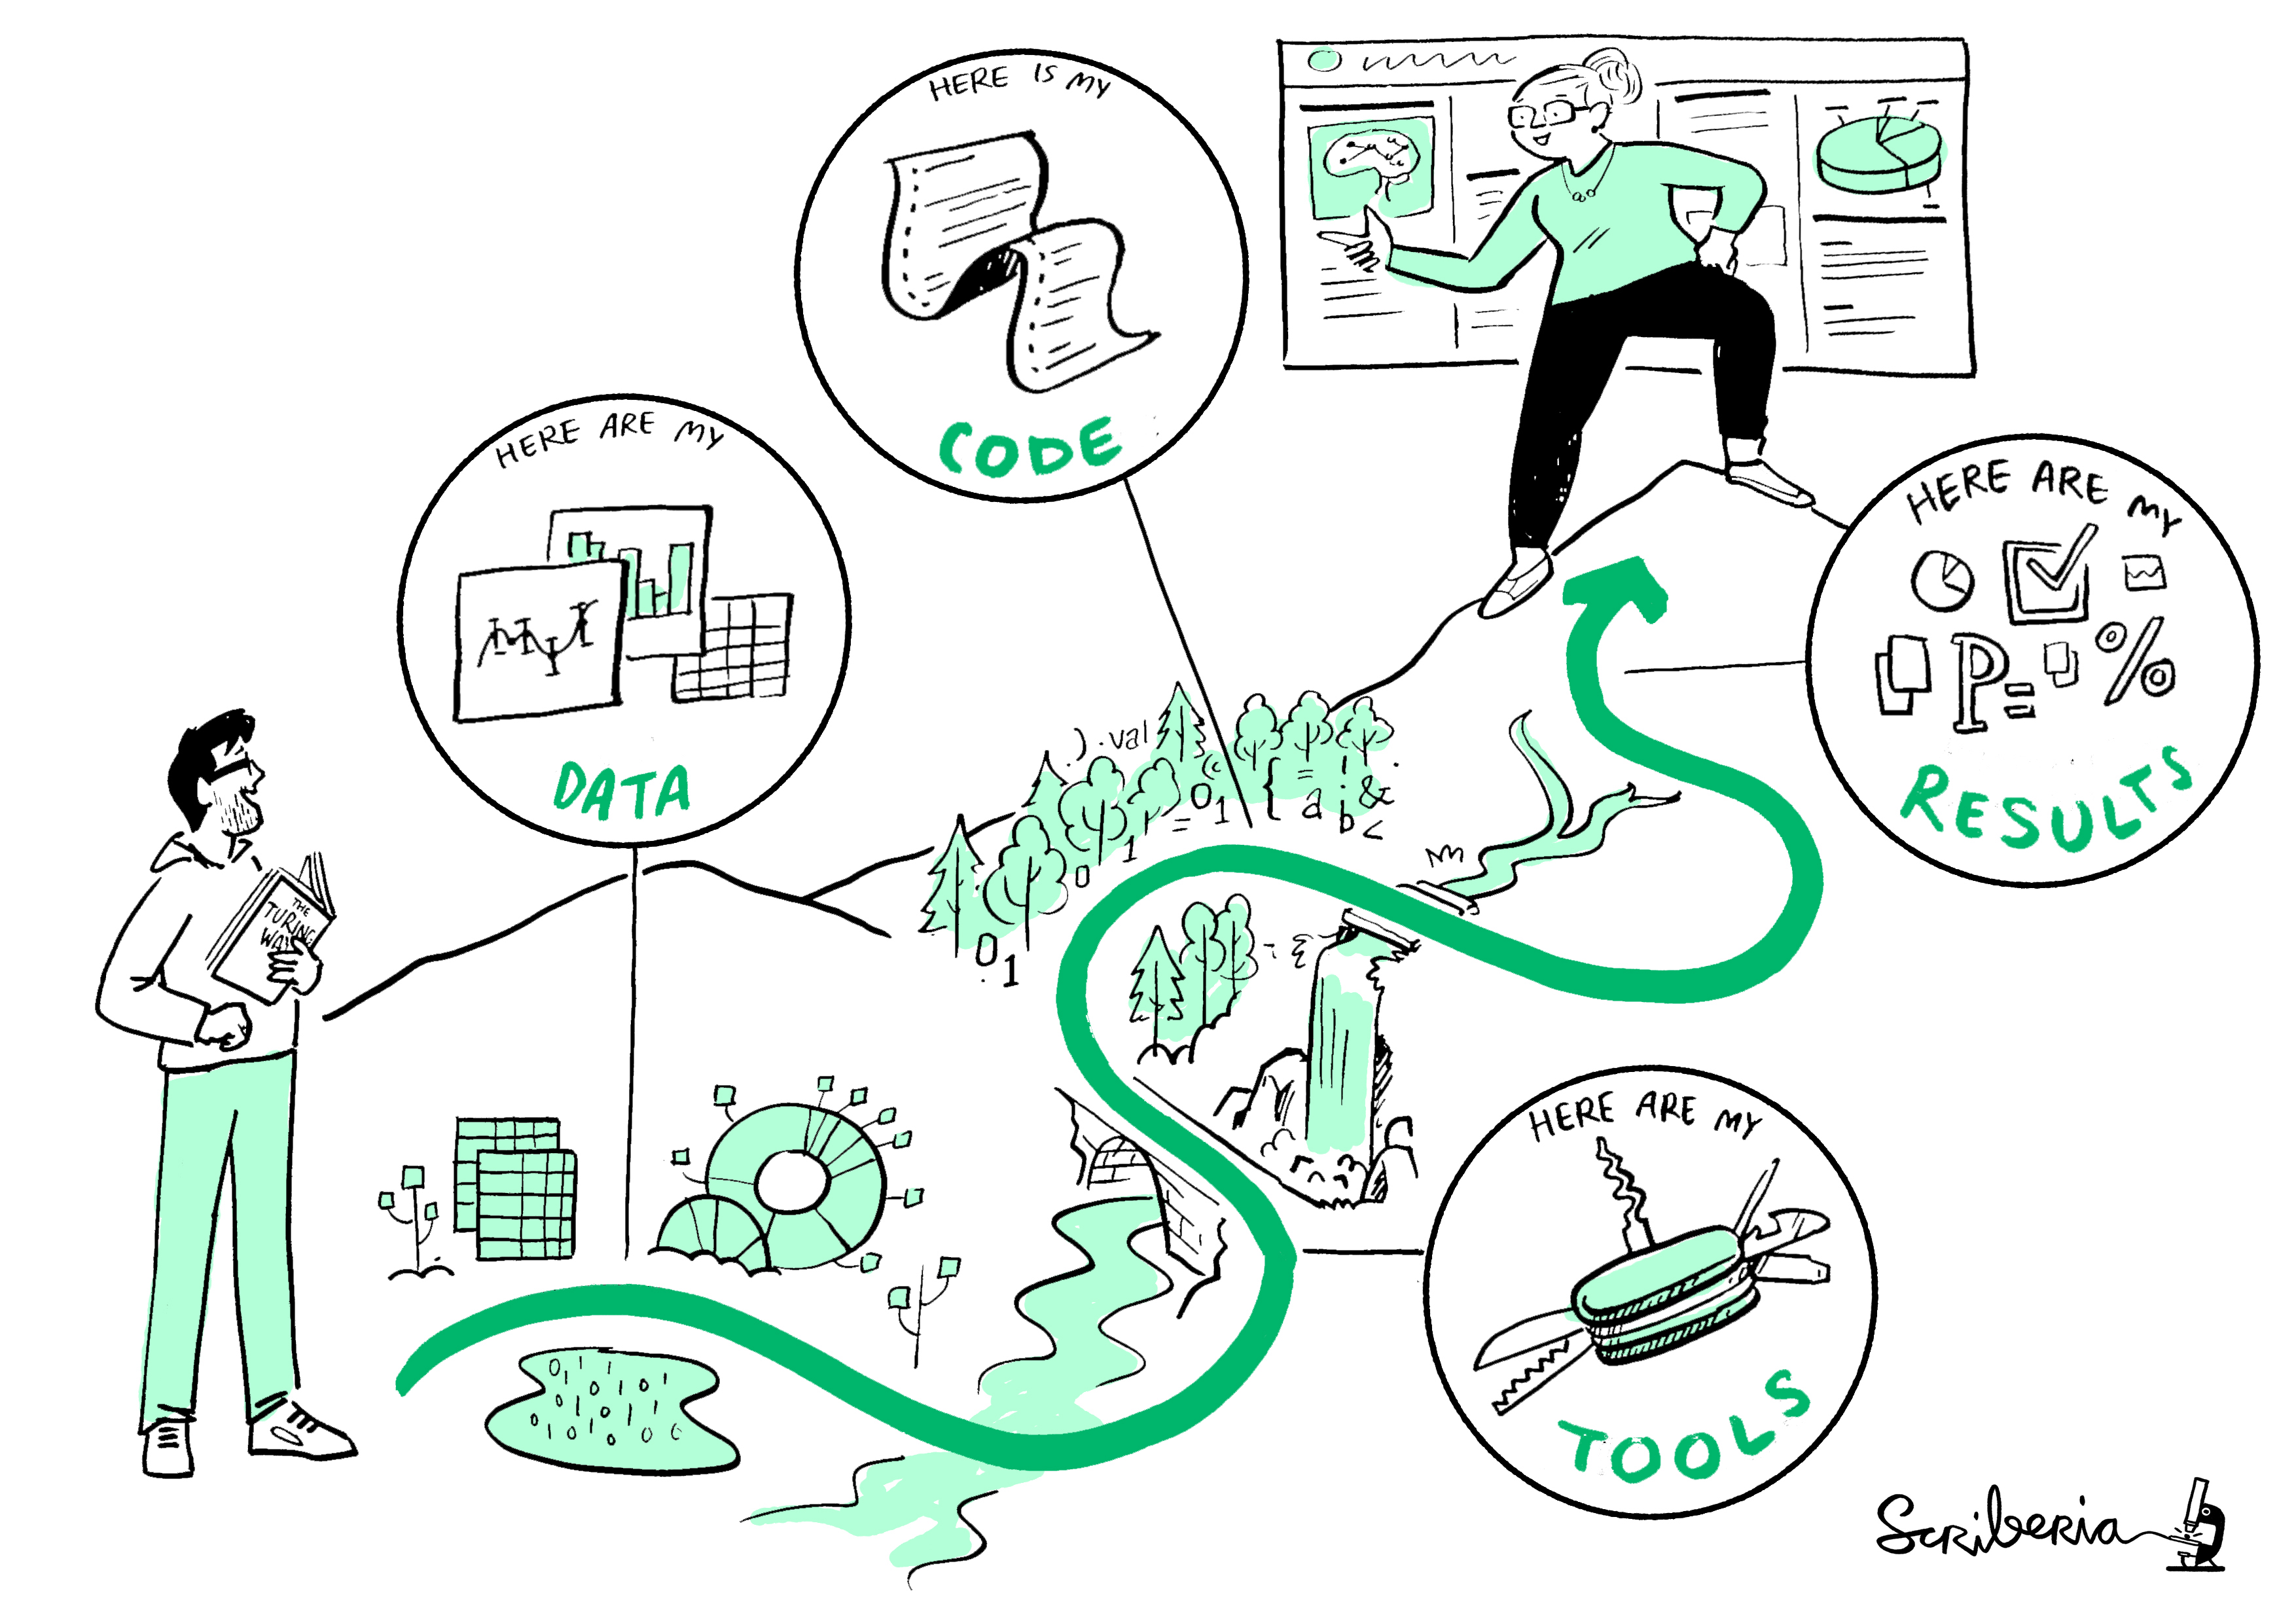
\includegraphics[width=.9\linewidth]{images/reproducibility.jpg}
\end{center}
\end{column}
\end{columns}
\end{frame}
\begin{frame}[label={sec:orgf9a1996},fragile]{Data Science Woes}
 \begin{columns}
\begin{column}{0.4\columnwidth}
\begin{itemize}
\item Version Control
\begin{itemize}
\item Git, SVN, Mercurial (\texttt{hg})
\end{itemize}
\item Collaboration
\begin{itemize}
\item Overleaf, Google Drive, OneDrive
\end{itemize}
\item Reproduce environments
\begin{itemize}
\item Docker, Conda, \alert{Nix}
\end{itemize}
\item Re-run analysis
\begin{itemize}
\item Luigi, any CWL runner
\end{itemize}
\end{itemize}
\end{column}

\begin{column}{0.6\columnwidth}
\begin{center}
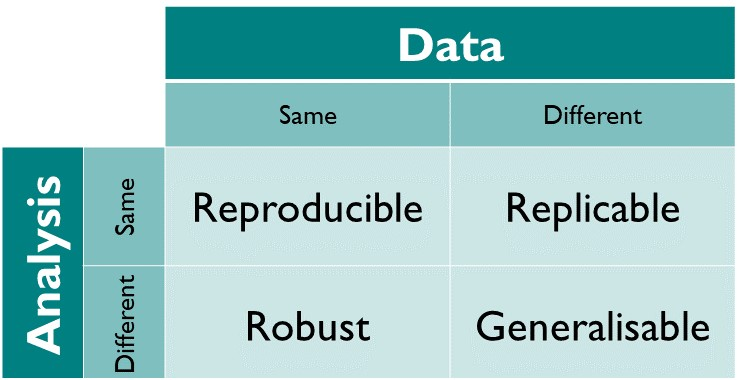
\includegraphics[width=.9\linewidth]{images/ReproducibleMatrix.jpg}
\end{center}
\end{column}
\end{columns}
\end{frame}

\begin{frame}[label={sec:org89be604},standout]{Section VI}
\section{Provenance and Clusters}
\begin{center}
  \Huge Provenance and Clusters
\end{center}
\end{frame}
\begin{frame}[label={sec:orge38abb4},fragile]{Cluster Woes}
 \begin{columns}
\begin{column}{0.4\columnwidth}
\begin{itemize}
\item No \texttt{docker}
\begin{itemize}
\item If lucky, will have \texttt{singularity}
\end{itemize}
\item No userspace support
\item Probably runs CentOS or something
\item Has a networked file system
\item Uses a resource queue
\begin{itemize}
\item Slurm, PBS
\end{itemize}
\item Might have support for \texttt{lmod}
\end{itemize}
\end{column}

\begin{column}{0.6\columnwidth}
\begin{center}
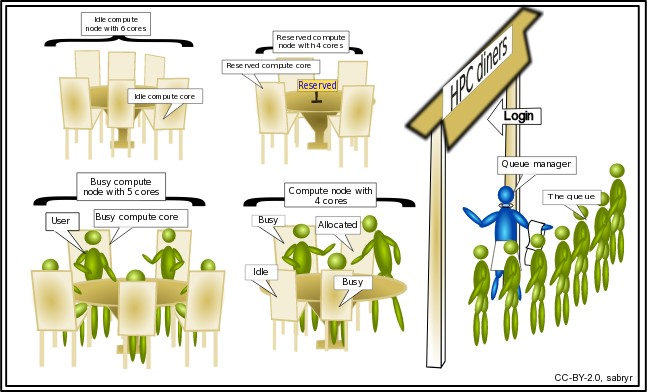
\includegraphics[width=.9\linewidth]{images/A_screenshot/2020-09-20_07-44-11_screenshot.png}
\end{center}
\end{column}
\end{columns}
\end{frame}

\begin{frame}[label={sec:org023aa20}]{Provenance}
\begin{columns}
\begin{column}{0.4\columnwidth}
\fullcite{communityTuringWayHandbook2019}

\begin{center}

\includegraphics[width=.9\linewidth]{images/A_block/2020-09-20_06-42-35_screenshot.png}
\end{center}
\end{column}

\begin{column}{0.6\columnwidth}
\begin{center}
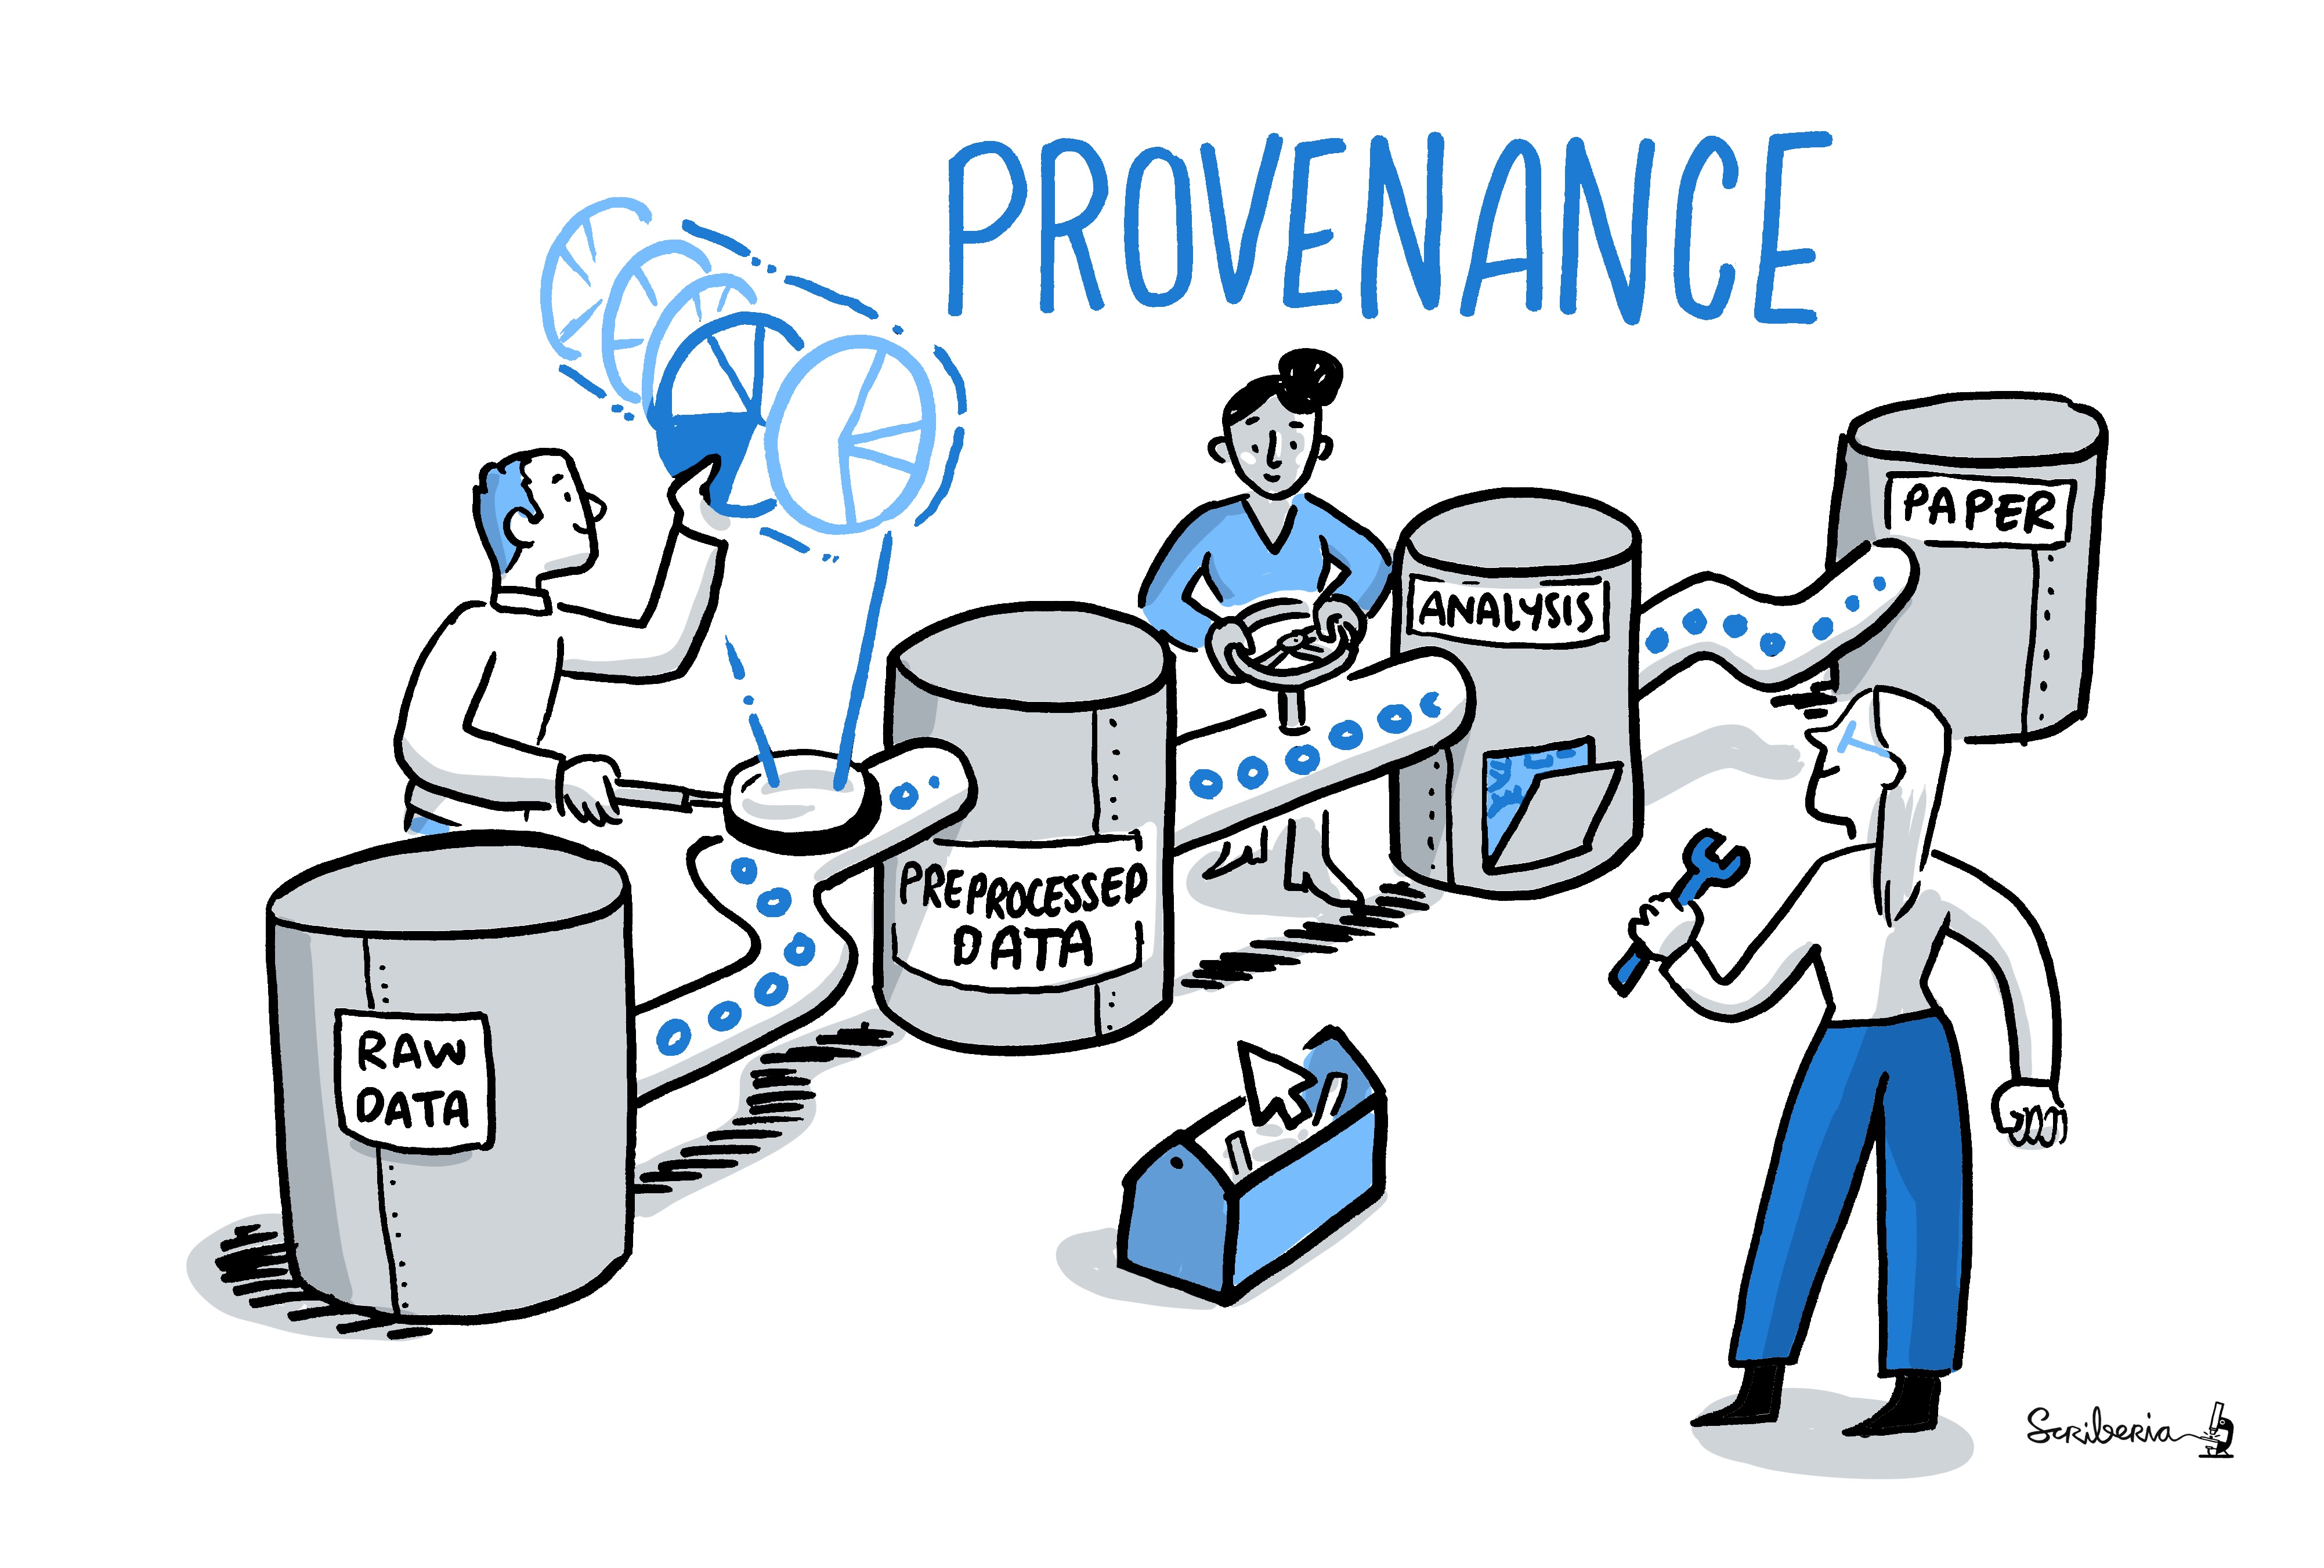
\includegraphics[width=.9\linewidth]{images/turingWay/Provenance.jpg}
\end{center}
\end{column}
\end{columns}
\end{frame}
\begin{frame}[label={sec:org8a7697a},fragile]{Setup Jupyter}
 \begin{columns}
\begin{column}{0.4\columnwidth}
\begin{itemize}
\item Prefer \texttt{conda}
\begin{itemize}
\item Export a \texttt{yml} with setup
\end{itemize}
\item Use \texttt{nvm}
\item Track provenance manually
\begin{itemize}
\item For plugins and setup
\end{itemize}
\item Consider \texttt{direnv}
\end{itemize}
\end{column}
\begin{column}{0.6\columnwidth}
\begin{minted}[bgcolor=white,breaklines=true,linenos=true,style=tango]{bash}
jupyter lab --generate-config
vim ~/.jupyter/jupyter_notebook_config.py
# Change c.NotebookApp.notebook_dir to a full path
\end{minted}
\end{column}
\end{columns}
\end{frame}
\begin{frame}[label={sec:org769cec6}]{Xeus Python}
\begin{columns}
\begin{column}{0.4\columnwidth}
\begin{itemize}
\item Best Jupyter debugger
\item Does not support all magics
\end{itemize}

\begin{center}

\includegraphics[width=.9\linewidth]{images/A_screenshot/2020-09-20_07-40-27_screenshot.png}
\end{center}
\end{column}


\begin{column}{0.6\columnwidth}
\begin{center}
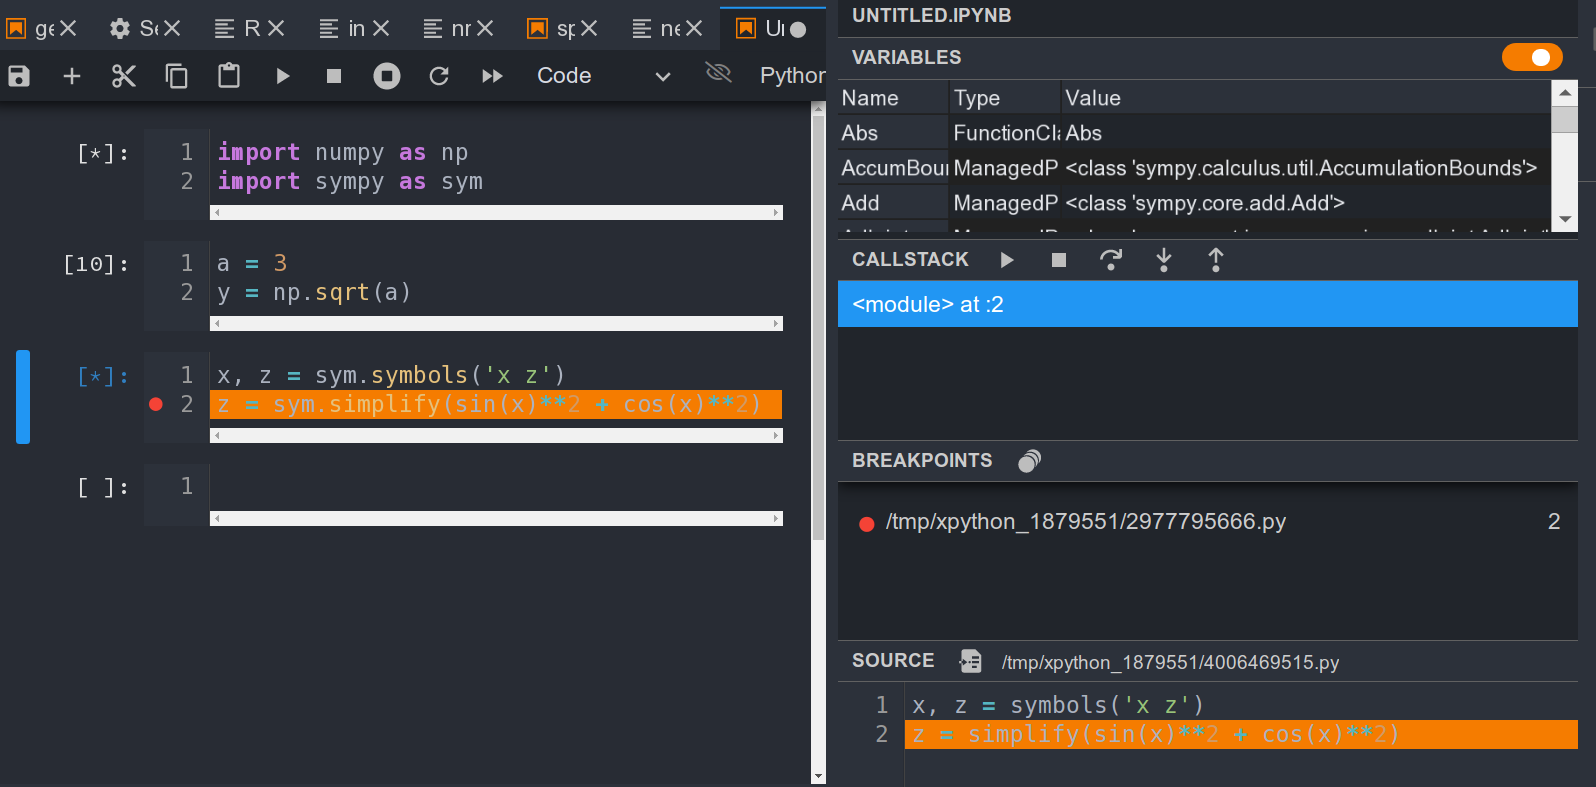
\includegraphics[width=.9\linewidth]{images/Xeus_Python/2020-09-20_07-39-12_screenshot.png}
\end{center}
\end{column}
\end{columns}
\end{frame}

\begin{frame}[label={sec:orgfbd1e57},fragile]{Reusing Notebooks}
 \begin{columns}
\begin{column}{0.5\columnwidth}
\begin{center}

\includegraphics[width=.9\linewidth]{images/logos/papermill_logo_wide.png}
\end{center}
\begin{block}{Papermill}
\begin{itemize}
\item Notebooks are \alert{functions}
\item Can be parameterized on the fly
\begin{itemize}
\item No need to refactor
\item Cells \alert{become} the analysis
\end{itemize}
\item Mostly supports integration tests
\end{itemize}
\end{block}
\end{column}

\begin{column}{0.4\columnwidth}
\begin{center}

\includegraphics[width=0.4\textwidth]{images/A_screenshot/2020-09-20_07-16-32_screenshot.png}
\end{center}

\begin{block}{Jupytext}
\begin{itemize}
\item Notebooks are literate snippets
\item Must refactor cells into functions
\item Supports testing more transparently
\begin{itemize}
\item Unit tests
\end{itemize}
\end{itemize}
\end{block}
\end{column}
\end{columns}
\begin{itemize}
\item Actually these work best together, especially as \texttt{papermill} can be called in \texttt{python} directly
\end{itemize}
\end{frame}
\begin{frame}[label={sec:org7048cc1},fragile]{Jupytext I}
 \begin{columns}
\begin{column}{0.4\columnwidth}
\begin{itemize}
\item Works best with version control
\begin{itemize}
\item Never commit an \texttt{.ipynb}!
\end{itemize}
\item Encourages functions
\begin{itemize}
\item Easier to unit-test later
\end{itemize}
\item Is literate
\begin{itemize}
\item Closer to \texttt{ipython} histories
\item Fits well with \texttt{orgmode} (via \texttt{pandoc})
\end{itemize}
\end{itemize}
\end{column}

\begin{column}{0.6\columnwidth}
\begin{center}
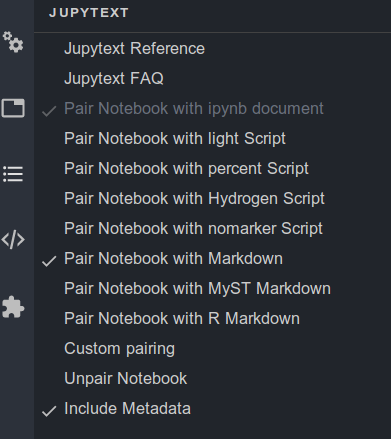
\includegraphics[width=0.6\textwidth]{images/A_screenshot/2020-09-20_07-11-59_screenshot.png}
\end{center}
\end{column}
\end{columns}
\end{frame}

\begin{frame}[label={sec:orgf4631c4}]{Jupytext II}
\begin{columns}
\begin{column}{0.5\columnwidth}
\begin{center}
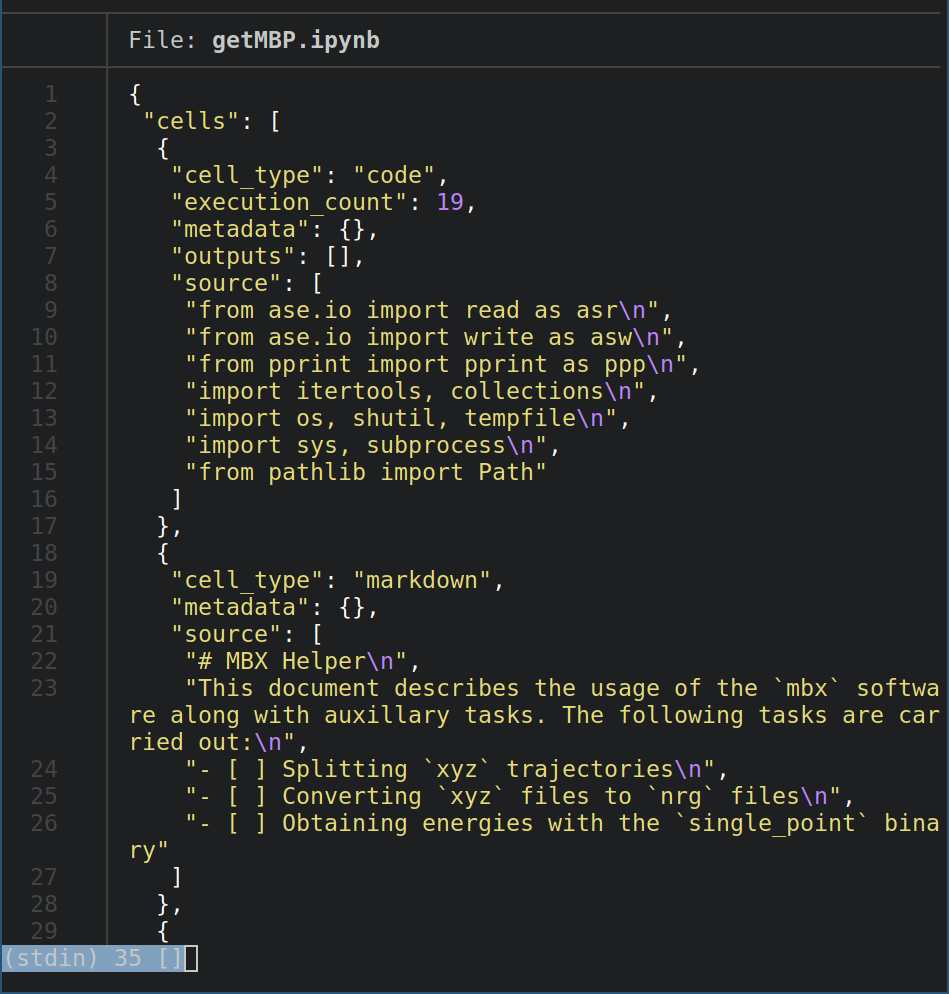
\includegraphics[width=0.9\textwidth]{images/A_screenshot/2020-09-20_09-01-21_screenshot.png}
\end{center}
\end{column}

\begin{column}{0.5\columnwidth}
\begin{center}
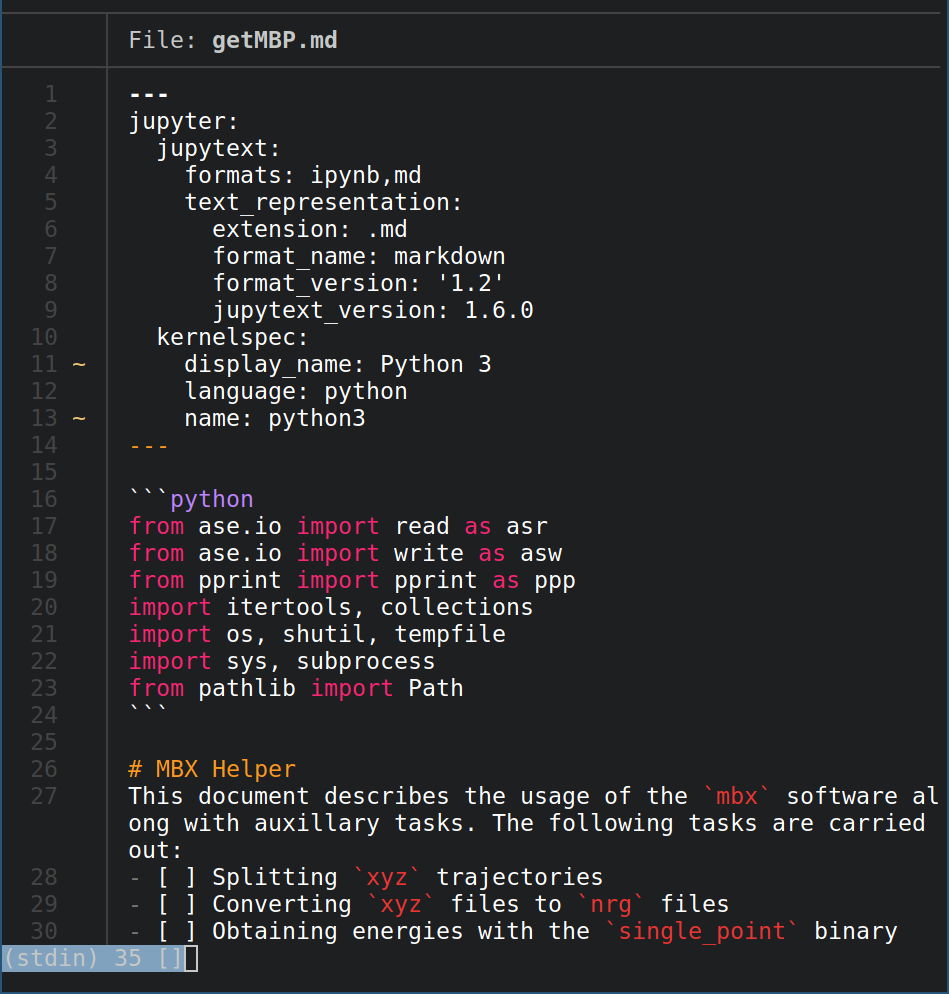
\includegraphics[width=0.9\textwidth]{images/A_screenshot/2020-09-20_09-01-40_screenshot.png}
\end{center}
\end{column}
\end{columns}
\end{frame}

\begin{frame}[label={sec:org05f967f},fragile]{Renku}
 \begin{columns}
\begin{column}{0.6\columnwidth}
\begin{itemize}
\item Has a Web-UI
\item Uses standard Git LFS under the hood
\item Generates CWL files for each command
\begin{itemize}
\item These become a provenance or lineage history
\item Image from renku docs
\end{itemize}
\end{itemize}

\begin{center}
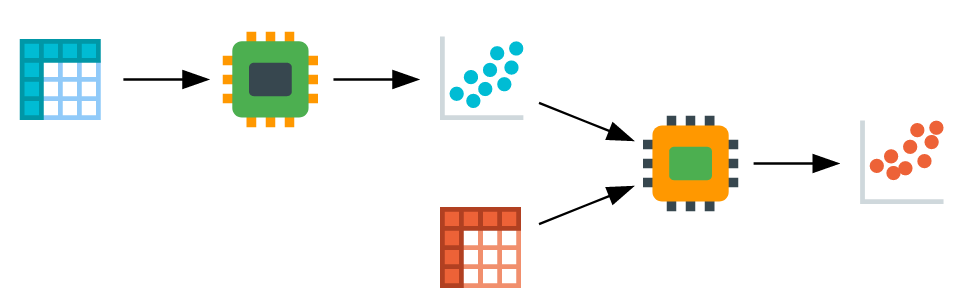
\includegraphics[width=.9\linewidth]{images/A_block/2020-09-20_06-55-30_screenshot.png}
\end{center}
\end{column}

\begin{column}{0.4\columnwidth}
\begin{quote}
Renku (連句 “linked verses”), is a Japanese form of popular collaborative linked verse poetry, written by more than one author working together.*
\end{quote}

—Wikipedia

\begin{minted}[bgcolor=white,breaklines=true,linenos=true,style=tango]{python}
renku run python run_analysis.py -i inputs -o outputs
\end{minted}
\end{column}
\end{columns}
\end{frame}
\begin{frame}[label={sec:org86cf683},standout]{Section VII}
\section{Towards the Future}
\begin{center}
  \Huge Towards the Future
\end{center}
\end{frame}

\begin{frame}[label={sec:org4907004},fragile]{Parting Practicalities}
 \begin{columns}
\begin{column}{0.6\columnwidth}
\begin{itemize}
\item Keep Jupyter \alert{impure}
\item Do \alert{not} rely on Colab
\item Always keep a plain-text version
\item Replace \alert{functions} with parameterized Jupyter notebooks
\item Reduce magics in parameterized notebooks
\begin{itemize}
\item Maximize Xeus where possible
\end{itemize}
\item Ask your sys-admins for \texttt{nix} or try a user-install
\begin{itemize}
\item Unsupported but try: \url{https://rgoswami.me/posts/local-nix-no-root/}
\end{itemize}
\end{itemize}
\end{column}
\begin{column}{0.4\columnwidth}
\begin{itemize}
\item \texttt{conda} should be used for \alert{global} installations
\begin{itemize}
\item Like Jupyter
\end{itemize}
\item Use \texttt{nix} derivations for actual environments
\item Use \texttt{renku} to track provenance per project
\begin{itemize}
\item Also tracks databases
\end{itemize}
\end{itemize}
\end{column}
\end{columns}
\end{frame}

\begin{frame}[label={sec:orgf77731b}]{Conclusions}
\begin{columns}
\begin{column}{0.6\columnwidth}
\begin{itemize}
\item Interactivity is here to stay
\begin{itemize}
\item Especially in data science
\end{itemize}
\item Jupyter notebooks are here to stay
\begin{itemize}
\item Scalable development is still possible
\end{itemize}
\item Nix ensures reproducible system dependencies
\end{itemize}

\begin{center}

\includegraphics[width=0.7\textwidth]{images/turingWay/BannerCongratulations.jpg}
\end{center}
\end{column}
\begin{column}{0.4\columnwidth}
\begin{itemize}
\item Meeting old-school TDD developers halfway is best
\end{itemize}
\begin{block}{Tools}
\begin{description}
\item[{Xeus Python}] PDB on steroids for Notebooks
\item[{Jupytext}] Version Control and literate programming
\item[{Papermill}] Notebooks-are-functions
\item[{Renku}] Write CWL without tears
\end{description}
\end{block}
\end{column}
\end{columns}
\end{frame}
\begin{frame}[allowframebreaks]{References}
\printbibliography
\end{frame}

\begin{frame}[label={sec:orge8418ab},standout]{End}
\begin{center}
  \Huge Thank you
\end{center}
\end{frame}
\end{document}
